\documentclass{beamer}

\usepackage{lads}

\usepackage{xcolor}

\definecolor{codegreen}{rgb}{0,0.6,0}
\definecolor{codegray}{rgb}{0.5,0.5,0.5}
\definecolor{codepurple}{rgb}{0.58,0,0.82}
\definecolor{backcolour}{rgb}{0.95,0.95,0.92}

\usepackage{listings}
\lstdefinestyle{mystyle}{
    backgroundcolor=\color{backcolour},   
    commentstyle=\color{codegreen},
    keywordstyle=\color{magenta},
    numberstyle=\tiny\color{codegray},
    stringstyle=\color{codepurple},
    basicstyle=\ttfamily\footnotesize,
    breakatwhitespace=false,         
    breaklines=true,                 
    captionpos=b,                    
    keepspaces=true,                 
    numbers=left,                    
    numbersep=5pt,                  
    showspaces=false,                
    showstringspaces=false,
    showtabs=false,                  
    tabsize=2
}

\lstset{style=mystyle}


\setbeamertemplate{navigation symbols}{}

\title{Linear Models II}
\date{}
\author{BIOE 210}

\begin{document}

\maketitle

\begin{frame}{Review: A \emph{noisy} linear system}

\begin{columns}
\begin{column}{0.3\textwidth}
\begin{center}
  \begin{tabular}{cccc}
    \toprule
    $x^\text{true}$ & $y^\text{true}$ \\
    \midrule
    0.07 & -0.05 \\
    0.16 & 0.40 \\
    0.48 & 0.66 \\
    0.68 & 0.65 \\
    0.83 & 1.12 \\
    \bottomrule
  \end{tabular}
\end{center}	
\end{column}

\begin{column}{0.7\textwidth}
\begin{center}
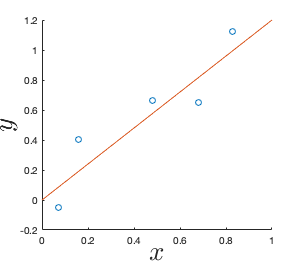
\includegraphics{simple_lin_scatter.png}
\end{center}	
\end{column}
\end{columns}
	
\end{frame}

\begin{frame}
\frametitle{A matrix formalism for linear models}
Let's write out one equation for each observation of the model $y = \beta_0 + \beta_1x$.
\begin{align*}
	-0.05 = \beta_0 + 0.07\beta_1 + \epsilon_1 \\
	0.40 = \beta_0 + 0.16\beta_1 + \epsilon_2 \\
	0.66 = \beta_0 + 0.48\beta_1 + \epsilon_3 \\
	0.65 = \beta_0 + 0.68\beta_1 + \epsilon_4 \\
	1.12 = \beta_0 + 0.83\beta_1 + \epsilon_5
\end{align*}

\pause
\[ \begin{pmatrix} -0.05\\ \phan0.40\\ \phan0.66\\ \phan0.65\\ \phan1.12 \end{pmatrix} = \begin{pmatrix} 1&0.07\\ 1&0.16\\ 1&0.48\\ 1&0.68\\ 1&0.83 \end{pmatrix} \vectwo{\beta_0}{\beta_1} + \begin{pmatrix} \epsilon_1\\ \epsilon_2\\ \epsilon_3\\ \epsilon_4\\ \epsilon_5 \end{pmatrix} \]
\pause
\[ \Vy = \V{X}\Vbeta+\Vepsilon \]	
\end{frame}

\begin{frame}
\frametitle{Solving the linear system}

A few points about $\Vy = \V{X}\Vbeta+\Vepsilon$:
\begin{itemize}
	\item The unknowns are \Vbeta, not \V{X}.
	\item The coefficient matrix \V{X}\ is called the \emph{model matrix}.
	\item The model matrix \V{X}\ is rarely square.
\end{itemize}

\pause
The solution to this system that minimizes the errors in \Vepsilon\ is 
\[ \Vbeta = \VX^+\Vy \]
where $\VX^+$ is the \emph{pseudoinverse} of \VX.
\end{frame}

\newcommand\Vone{\V{1}}

\begin{frame}{The intercept}

The linear model
\[ \Vy = \beta_0 + \beta_1\Vx_1 + \beta_2\Vx_2 + \Vepsilon \]
has intercept (or \emph{grand mean}) $\beta_0$.

\pause
\medskip
Really, we should write the model as
\[ \Vy = \beta_0\Vone + \beta_1\Vx_1 + \beta_2\Vx_2 + \Vepsilon. \]

\pause
Or, in vector form
\[ \Vy = \begin{mex}\Vone & \Vx_1 & \Vx_2\end{mex}\vecthree{\beta_0}{\beta_1}{\beta_2} + \Vepsilon. \]

\end{frame}

\begin{frame}{Models without an intercept}

If we wanted to fit a model without an intercept, we would write 
\[ \Vy = \begin{mex}\Vx_1 & \Vx_2\end{mex}\vectwo{\beta_1}{\beta_2} + \Vepsilon. \]

\pause
Why would we not want an intercept?
\begin{itemize}
	\item When all inputs $\Vx_i = 0$, the response $y = \beta_0$.
	\pause
	\item If we know our system has zero response without an input, we don't include an intercept.
	\pause
	\item This is rare, so most models include an intercept.
\end{itemize}

\end{frame}

\begin{frame}{Prediction vs. Inference}

\textbf{Prediction} uses a model to find the response of inputs we've never seen before.

\medskip
\textbf{Inference} uses a model to understand what inputs determine the response.
	
\end{frame}

\begin{frame}{How accurate are a model's predictions?}

\pause
Our training data include a design matrix $\VX$ and a vector of responses $\Vy$. Each has $n$ observations (rows).

\pause
\medskip
We fit the model $\Vy = \VX\Vbeta + \Vepsilon$ to find the best parameters $\Vbeta$.

\pause
\medskip
We feed the training data back into the model to find the residuals: 
\begin{align*}
	\Vepsilon &= \Vy - \VX\Vbeta \\
		&= \Vy^\text{true} - \Vy^\text{pred}
\end{align*}

\pause
\medskip
We quantify the accuracy using the \emph{root mean squared error} of the residuals.
\[ \text{RMSE} = \sqrt{\frac{1}{n}\sum_{i=1}^n\left( y^\text{true}_i - \ypred_i \right)^2} \]
	
\end{frame}

\begin{frame}{Prediction intervals}

A model's predictions should be reported $\pm$ the RMSE.

\pause
\medskip
The 95\% confidence interval of a prediction is $\pm 2\times\text{RMSE}$.

\pause
\medskip
\textbf{Example:} A model to predict pulse rate has RMSE of 12~bpm. If the model predicts 68~bpm for a patient, the 95\% confidence interval is
\[ [68-2\times12,\, 68+2\times12] = [44,92]\,\,\text{bpm} \]

\pause
\medskip
Remember: If you transformed your model, the RMSE will be in the transformed units!

\end{frame}

\begin{frame}{Model inference}

Model inference involves asking two questions about each of the models inputs.
\begin{enumerate}
	\item How large of an effect does this input have on the output?
	\item How confident are we in our estimate of this effect?
\end{enumerate}

\medskip
\pause
Consider the two input model
\[ \Vy = 1.2 - 3.6\Vx_1 + 0.8\Vx_2 + \Vepsilon. \]

\pause
The parameters $-3.6$ and $0.8$ are called \emph{effect sizes}.

\medskip
\pause
\begin{itemize}
	\item A unit change in variable $\Vx_1$ would \emph{decrease} the response by 3.6 units. 
	\item A unit change in $\Vx_2$ would \emph{increase} the response by 0.8 units.
\end{itemize}

\end{frame}

\begin{frame}{How sure are we of the effect sizes?}

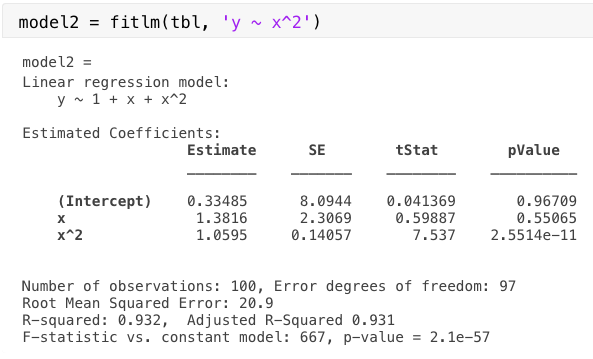
\includegraphics{fitlm}

\end{frame}

\begin{frame}{What does this $p$-value mean?}

\begin{itemize}
	\item A low $p$-value indicates that an effect of this size was unlikely to occur randomly.
	\item It also means the confidence interval \emph{excludes} zero, so we reject the hypothesis that the true effect is zero.
	\pause
	\item It does \textbf{not} mean that the effect is practically significant or important. (That's up to the effect size.)
\end{itemize}
	
\end{frame}

\begin{frame}

\begin{center}

\includegraphics[width=0.7\textwidth]{online-meet}
\end{center}

\begin{quotation}\small
	For respondents categorized as currently married at the time of the survey, we examined marital satisfaction. Analyses indicated that currently married respondents who met their spouse on-line reported higher marital satisfaction (M = 5.64, SE = 0.02, $n$ = 5,349) than currently married respondents who met their spouse off-line (M = 5.48, SE = 0.01, $n$ = 12,253; mean difference = 0.18, $F_{(1, 17,601)} = 46.67$, $P < 0.001$).
\end{quotation}
	
\end{frame}

\newcommand\mathcolon{{:}}

\begin{frame}
\frametitle{Interactions}	

Imagine we're modeling the response ($y$) from two input variables, $\Vx_1$ and $\Vx_2$. The simplest model is

\[ y = \beta_1\Vx_1 + \beta_2\Vx_2 + \epsilon \]

\pause
The coefficient $\beta_1$ measures the effect of $\Vx_1$ and $\beta_2$ measures the effect of $\Vx_2$. These effects are \textbf{independent}.

\bigskip
\pause
What is there is another effect that depends on both $\Vx_1$ and $\Vx_2$? This is an \textbf{interaction} between $\Vx_1$ and $\Vx_2$.
\end{frame}

\begin{frame}
\frametitle{How do we model interactions?}

We model the interaction of $\Vx_1$ and $\Vx_2$ using the product of these variables.
\[ y = \beta_1\Vx_1 + \beta_2\Vx_2 + \beta_{12}\Vx_1\mathcolon\Vx_2 + \epsilon \]

The coefficient $\beta_{12}$ is the effect size of the interaction.

\pause
\bigskip
Why do we multiply $\Vx_1$ and $\Vx_2$? There are at least two ways to interpret this term.
\end{frame}

\begin{frame}
\frametitle{The coded factor interpretation}

Often we set up design matrices using \textbf{coded variables}. If we're testing the variable at two levels, we code the variable as ``on/off''~($\{0,1\}$) or ``low/high''~($\{-1,+1\}$).

\pause
\bigskip
\begin{columns}
\begin{column}{0.55\textwidth}
on/off $\rightarrow$ interaction when both ``on''
\begin{center}
\begin{tabular}{cc|c}
	$\Vx_1$ & $\Vx_2$ & $\Vx_1\mathcolon \Vx_2$ \\
	\hline
	0 & 0 & 0 \\
	0 & 1 & 0 \\
	1 & 0 & 0 \\
	1 & 1 & 1
\end{tabular}
\end{center}
\end{column}

\pause
\begin{column}{0.5\textwidth}
high/low $\rightarrow$ interaction when both ``high'' or both ``low''
\begin{center}
\begin{tabular}{cc|c}
	$\Vx_1$ & $\Vx_2$ & $\Vx_1\mathcolon \Vx_2$ \\
	\hline
	$-1$ & $-1$ & $+1$ \\
	$-1$ & $+1$ & $-1$ \\
	$+1$ & $-1$ & $-1$ \\
	$+1$ & $+1$ & $+1$
\end{tabular}
\end{center}
\end{column}
\end{columns}

\end{frame}

\begin{frame}
\frametitle{The augmented slope interpretation}

We can also interpret the interaction as one variable changing the effect of the other variable.

\begin{align*}
	y &= \beta_1\Vx_1 + \beta_2(\Vx_1)\mathcolon\Vx_2 + \epsilon \\
	 &= \beta_1\Vx_1 + (\beta_2 + \beta_{12}\Vx_1)\mathcolon \Vx_2 + \epsilon \\
	 &= \beta_1\Vx_1 + \beta_2\Vx_2 + \beta_{12}\Vx_1\mathcolon \Vx_2 + \epsilon
\end{align*}
\end{frame}

\begin{frame}
\frametitle{Things to remember about interactions}

\begin{itemize}
	\item Interaction are modeled as the product of variables.
	\item The interaction effect is ``above and beyond" the independent effects (synergy/super-additivity, antagonism/sub-additivity).
	\item Higher-order interactions are possible (e.g. $\Vx_1\Vx_2\Vx_3$), but these are rare.
\end{itemize}
\end{frame}




\end{document}
